\section*{Cycle 1 Experiment 3}

\section{\Large{Process and Thread}}

\subsection{Aim}
\large To familiarize and implement programs related to process and thread.

\subsection{Theory}
\textbf{Thread: }
A thread is a path of execution within a process. It has its own program counter that keeps track of which instruction to execute next, system registers which hold its current working variables, and a stack which contains the execution history. It shares with its peer threads few information like code segment, data segment and open files.
\\
\\
\textbf{Process: }
A process can be defined as an entity which represents the basic unit of work to be implemented in the system. Basically speaking, a process is a program in execution. For example, the original code we write and binary code which we process are both programs. When we actually run the binary code, it becomes a process.
\\
\\
\textbf{Differences: }
A thread can do anything a process can do. But a process can consist of multiple threads, and hence thread could be considered a ‘lightweight’ process. Threads are used for small tasks, whereas processes are used for more ‘heavyweight’ tasks – basically the execution of applications. Another difference between a thread and a process is that threads within the same process share the same address space, whereas different processes do not. This allows threads to read from and write to the same data structures and variables, and also facilitates communication between threads. Communication between processes – also known as IPC, or inter-process communication is quite difficult and resource-intensive.

\subsection{Algorithm}
\begin{verbatim}
Algorithm for creating threads

1 START
2 Let n = 3
3 Procedure ∗ThreadFunction (void ∗arg)
4 BEGIN
5 Print some random text
6 sleep(1)
7 print Thread ID, Process ID
8 END ThreadFunction
9 Create pthread t
10 Let j = fork( )
11 IF j = 0 THEN //child process
12 BEGIN − for i < n //create thread for child process
13 CALL pthreadcreate(&t, NULL, ThreadFunction, i ) and increment i by 1
14 END − for
15 ELSE then // parent process
16 BEGIN − for i < n //create parent thread for process
17 CALL pthreadcreate(&t, NULL, ThreadFunction, i ) and increment i by 1
18 END − for
19 ENDIF
20 STOP   
\end{verbatim}

\subsection{Code}
\begin{verbatim}
#include<stdio.h>
#include<stdlib.h>
#include<unistd.h>
#include<pthread.h>
#include<sys/types.h>

const int n=3;

void *ThreadFunction(void *arg){
    printf("*Bon Jour!*\n");  //some random text
    sleep(1);
    printf("ThreadID: %d\t Process: %d\n",(void *)arg, getpid());
}

int main(){
    int i;
    pthread_t t;
    int j = fork();
    wait();
    if(j == 0){
        printf("Child Thread\n");
        for(i = 0; i < n; i++)
            pthread_create(&t, NULL, ThreadFunction, (void *)i);
    }
    else{
        printf("Parent Thread\n");
        for(i = 0; i < n; i++)
            pthread_create(&t, NULL, ThreadFunction, (void *)i);
    }

    pthread_exit(NULL);
    return 0;
}
\end{verbatim}
\newpage
\subsection{Output}
\begin{figure}[h]
            \centering
            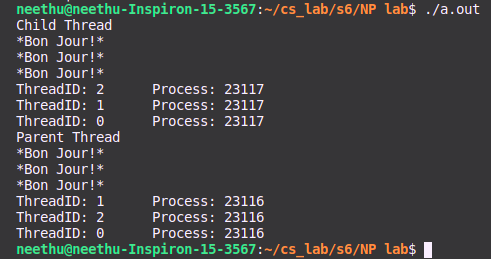
\includegraphics[scale=0.9]{img/e3.png}
\end{figure}
        
\subsection{Result}
Implemented the program for creating threads using C language in Ubuntu 18.04 with kernel and the above outputs were obtained.